\documentclass{article}

% Language setting
% Replace `english' with e.g. `spanish' to change the document language
\usepackage[UTF8]{ctex}

% Set page size and margins
% Replace `letterpaper' with `a4paper' for UK/EU standard size
\usepackage[letterpaper,top=2cm,bottom=2cm,left=3cm,right=3cm,marginparwidth=1.75cm]{geometry}

% Useful packages
\usepackage{amsmath}
\usepackage{graphicx}
\usepackage[colorlinks=true, allcolors=blue]{hyperref}

\title{MA206 Homework5}
\author{12110120 赵钊}

\begin{document}
\maketitle


\section{第1题}

\subsection{1}
\subsubsection{a}
\begin{table}[!h]
\begin{center}
\begin{tabular}{|c|c|c|c|}
    \hline
    $V$ & $P$ & $log V$ & $log P$ \\
    \hline
    341948 &	4.81	&12.74241396	&1.570697084\\
    \hline
1092759 &	5.88 &	13.90421625 &	1.771556762\\
\hline
5491 &	3.31 &	8.610865667 &	1.196948189\\
\hline
49375 &	4.9	 & 10.8071995 &	1.589235205\\
\hline
1340000 &	5.62 &	14.10818017 &	1.726331664\\
\hline
365 &	2.76 &	5.899897354 &	1.01523068\\
\hline
2500	& 2.27	 & 7.824046011 &	0.819779831\\
\hline
78200 &	3.85 &	11.26702493 &	1.348073148\\
\hline
867023 &	5.21 &	13.67282078 &	1.650579856\\
\hline
14000 &	3.70 & 	9.546812609 &	1.30833282\\
\hline
23700	 & 3.27 &	10.07323033 &	1.184789985\\
\hline
70700 &	4.31 &	11.16620085 &	1.460937904\\
\hline
304500 &	4.42 &	12.62642637 &	1.486139696\\
\hline 
138000 &	4.39 &	11.83500896 &	1.479329227\\
\hline
2602000 &	5.05 &	14.77179094 &	1.619388243\\
\hline
\end{tabular}
\caption{\label{demo-table}数据处理}
\end{center}
\end{table}

数据如上表。

\newpage

\subsubsection{b}
\begin{figure}[!h]
    \centering
    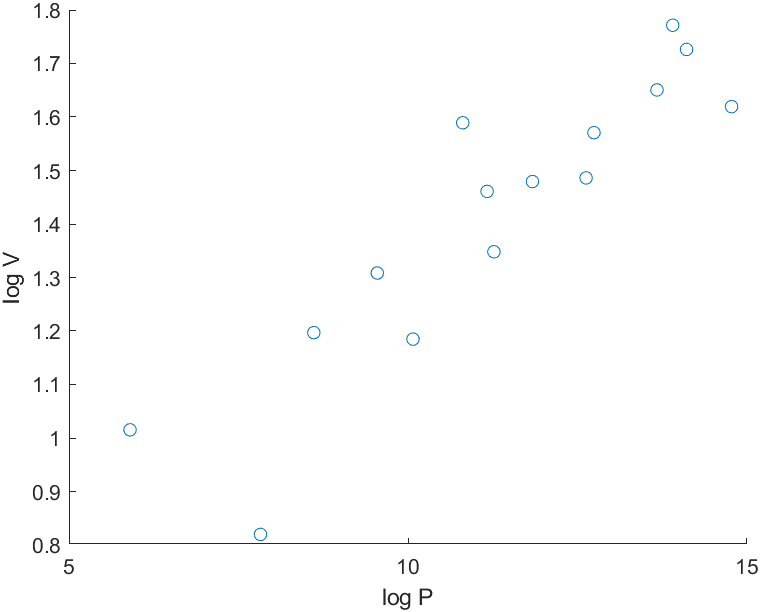
\includegraphics[width=0.5\textwidth]{pic/hw5_1.png}
    \caption{散点图}
\end{figure}

\subsubsection{c - e}
拟合得到一次函数如下:

\begin{figure}[!h]
    \centering
    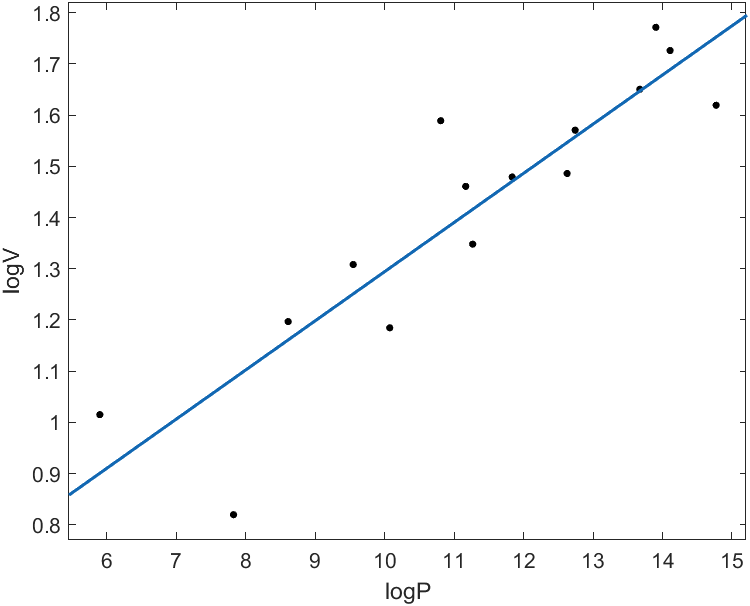
\includegraphics[width=0.5\textwidth]{pic/hw5_2.png}
    \caption{拟合图}
\end{figure}

其函数表达式为
\[log V = 0.096log P + 0.3343 \quad (R^2 = 0.8131)\]

\subsubsection{f}
对(e)得到的函数表达式同时取$e^{(.)}$

得到
\[V = 1.397P^{0.096}\]

\newpage

\subsection{2}

\begin{figure}[!h]
    \centering
    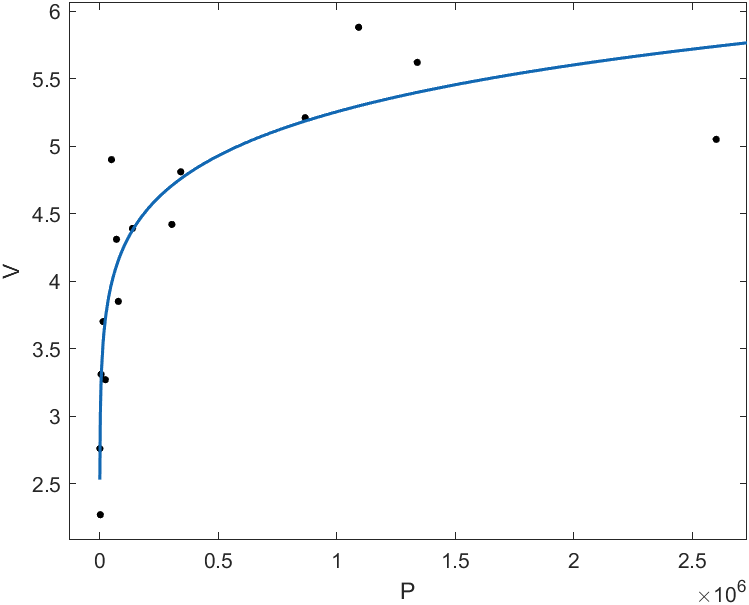
\includegraphics[width=0.5\textwidth]{pic/hw5_3.png}
    \caption{拟合图}
\end{figure}


\subsection{3 - 4}

\begin{table}[!h]
\begin{center}
\begin{tabular}{|c|c|c|c|}
    \hline
    Location & $V$ & $V_p$ & $|V-V_p|$ \\
    \hline
    1 &	4.81	& 4.747408168 & 0.062591832\\
\hline
2 &	5.88 &	5.307557988 &	0.572442012\\
\hline
3 &	3.31 &	3.193029601 &	0.116970399\\
\hline
4 &	4.9	 & 3.942512587 &	0.957487413\\
\hline
5 &	5.62 &	5.412506947 &	0.207493053\\
\hline
6 &	2.76 &	2.461367836 &	0.298632164\\
\hline
7	& 2.27	 & 2.960728928 &	0.690728928\\
\hline
8 &	3.85 &	4.120446261 &	0.270446261\\
\hline
9 &	5.21 &	5.190955974 &	0.019044026\\
\hline
10 &	3.70 & 	3.493210023 &	0.206789977\\
\hline
11	 & 3.27 &	3.674279987  &	0.404279987\\
\hline
12 &	4.31 &	4.080756395 &	0.229243605\\
\hline
13 &	4.42 &	4.694839897 &	0.274839897\\
\hline 
14 &	4.39 &	4.351357828 &	0.038642172\\
\hline
15 &	5.05 &	5.76853997 &	0.71853997\\
\hline
\end{tabular}
\caption{\label{demo-table}数据处理}
\end{center}
\end{table}

残差平均值为
$\frac{1}{15} \sum|V-V_p| = 0.338$

V的真实值均值为
$\frac{1}{15} \sum V = 4.25$

误差比率为$\frac{0.338}{4.25} = 7.9\%$

拟合精确度仍有提升空间。

\newpage


\section{第2题}

\subsection{a}
使用拉格朗日插值法对15组数据(设为$(x_0,y_0)$,$(x_1,y_1)$,...,$(x_{14},y_{14})$)进行拟合,拟合成为最高次项为14的多项式,其表达式为
\[f(x) = \sum_{n=0}^{14} y_n L_n(x)\]

其中
\[L_k(x) = \frac{(x-x_0)(x-x_1)...(x-x_{k-1})(x-x_{k+1})...(x-x_{14})}{(x_k-x_0)(x_k-x_1)...(x_k-x_{k-1})(x_k-x_{k+1})...(x_k-x_{14})}\]

使用多项式拟合的弊端在于,用拟合函数进行预测效果较差,原因是其头部和尾部可能不收敛,从而使预测结果偏差甚远。

\subsection{b}
同(a)的做法,本题对14组数据进行最高次项为13的多项式拟合,数据如下

\begin{table}[!h]
\begin{center}
\begin{tabular}{c|c c c c c c c c c c c c c c}
    
    i & 0 & 1 & 2 & 3 & 4 & 5 & 6 & 7 & 8 & 9 & 10 & 11 & 12 & 13 \\
    \hline
    $x_i$ & 17 & 19 & 20 & 22 & 23 & 25 & 31 & 32 & 33 & 36 & 37 & 38 & 39 & 41  \\
    
    $y_i$ &  19 & 25 & 32 & 51 & 57 & 71 & 141 & 123 & 187 & 192 & 205 & 252 & 248 & 294  \\
    
\end{tabular}
\caption{\label{demo-table}数据}
\end{center}
\end{table}


\section{第3题}

\subsection{1}

对数据进行多次差分,差分过程如下

\begin{table}[!h]
\begin{center}
\begin{tabular}{c|c c c c c c c c}
    x & 0 & 1 & 2 & 3 & 4 & 5 & 6 & 7  \\
    \hline
    y & 2 & 8 & 24 & 56 & 110 & 192 & 308 & 464 \\
\end{tabular}
\caption{\label{demo-table}数据}
\end{center}
\end{table}

\begin{table}[!h]
\begin{center}
\begin{tabular}{c|c c c c c c c c}
    $\Delta x$ & 0 & 1 & 2 & 3 & 4 & 5 & 6  \\
    \hline
    y & 6 & 16 & 32 & 54 & 82 & 116 & 156 \\
\end{tabular}
\caption{\label{demo-table}一阶差分}
\end{center}
\end{table}

\newpage

\begin{table}[!h]
\begin{center}
\begin{tabular}{c|c c c c c c c c}
    $\Delta^2 x$ & 0 & 1 & 2 & 3 & 4 & 5  \\
    \hline
    y & 10 & 16 & 22 & 28 & 34 & 40 \\
\end{tabular}
\caption{\label{demo-table}二阶差分}
\end{center}
\end{table}

\begin{table}[!h]
\begin{center}
\begin{tabular}{c|c c c c c c c c}
    $\Delta^3 x$ & 0 & 1 & 2 & 3 & 4  \\
    \hline
    y & 6 & 6 & 6 & 6 & 6 \\
\end{tabular}
\caption{\label{demo-table}三阶差分}
\end{center}
\end{table}

观察到三阶差分的插值已相等,因此多项式拟合最高次项为3次。



\subsection{2}

对数据进行差分,差分过程如下

\begin{table}[!h]
\begin{center}
\begin{tabular}{c|c c c c c c c c}
    x & 0 & 1 & 2 & 3 & 4 & 5 & 6 & 7  \\
    \hline
    y & 23 & 48 & 73 & 98 & 123 & 148 & 173 & 198 \\
\end{tabular}
\caption{\label{demo-table}数据}
\end{center}
\end{table}

\begin{table}[!h]
\begin{center}
\begin{tabular}{c|c c c c c c c c}
    $\Delta x$ & 0 & 1 & 2 & 3 & 4 & 5 & 6  \\
    \hline
    y & 25 & 25 & 25 & 25 & 25 & 25 & 25 \\
\end{tabular}
\caption{\label{demo-table}一阶差分}
\end{center}
\end{table}

观察到一阶差分的插值已相等,因此多项式拟合最高次项为1次。


\subsection{3}

对数据进行差分,差分过程如下

\begin{table}[!h]
\begin{center}
\begin{tabular}{c|c c c c c c c c}
    x & 0 & 1 & 2 & 3 & 4 & 5 & 6 & 7  \\
    \hline
    y & 7 & 15 & 33 & 61 & 99 & 147 & 205 & 273 \\
\end{tabular}
\caption{\label{demo-table}数据}
\end{center}
\end{table}

\begin{table}[!h]
\begin{center}
\begin{tabular}{c|c c c c c c c c}
    $\Delta x$ & 0 & 1 & 2 & 3 & 4 & 5 & 6  \\
    \hline
    y & 8 & 18 & 28 & 38 & 48 & 58 & 68 \\
\end{tabular}
\caption{\label{demo-table}一阶差分}
\end{center}
\end{table}

\newpage

\begin{table}[!h]
\begin{center}
\begin{tabular}{c|c c c c c c c c}
    $\Delta^2 x$ & 0 & 1 & 2 & 3 & 4 & 5  \\
    \hline
    y & 10 & 10 & 10 & 10 & 10 & 10 \\
\end{tabular}
\caption{\label{demo-table}二阶差分}
\end{center}
\end{table}

观察到二阶差分的插值已相等,因此多项式拟合最高次项为2次。


\subsection{4}

对数据进行多次差分,过程如下

\begin{table}[!h]
\begin{center}
\begin{tabular}{c|c c c c c c c c}
    x & 0 & 1 & 2 & 3 & 4 & 5 & 6 & 7  \\
    \hline
    y & 1 & 4.5 & 20 & 90 & 403 & 1808 & 8103 & 36316 \\
\end{tabular}
\caption{\label{demo-table}数据}
\end{center}
\end{table}

\begin{table}[!h]
\begin{center}
\begin{tabular}{c|c c c c c c c c}
    $\Delta x$ & 0 & 1 & 2 & 3 & 4 & 5 & 6  \\
    \hline
    y & 3.5 & 15.5 & 70 & 313 & 1405 & 6295 & 28213 \\
\end{tabular}
\caption{\label{demo-table}一阶差分}
\end{center}
\end{table}

\begin{table}[!h]
\begin{center}
\begin{tabular}{c|c c c c c c c c}
    $\Delta^2 x$ & 0 & 1 & 2 & 3 & 4 & 5  \\
    \hline
    y & 12 & 54.5 & 243 & 1092 & 4890 & 21918 \\
\end{tabular}
\caption{\label{demo-table}二阶差分}
\end{center}
\end{table}

\begin{table}[!h]
\begin{center}
\begin{tabular}{c|c c c c c c c c}
    $\Delta^3 x$ & 0 & 1 & 2 & 3 & 4  \\
    \hline
    y & 42.5 & 188.5 & 849 & 3798 & 17028  \\
\end{tabular}
\caption{\label{demo-table}三阶差分}
\end{center}
\end{table}

\begin{table}[!h]
\begin{center}
\begin{tabular}{c|c c c c c c c c}
    $\Delta^4 x$ & 0 & 1 & 2 & 3  \\
    \hline
    y & 146 & 660.5 & 2949 & 13230  \\
\end{tabular}
\caption{\label{demo-table}四阶差分}
\end{center}
\end{table}

\begin{table}[!h]
\begin{center}
\begin{tabular}{c|c c c c c c c c}
    $\Delta^5 x$ & 0 & 1 & 2  \\
    \hline
    y & 514.5 & 2288.5 & 10281  \\
\end{tabular}
\caption{\label{demo-table}五阶差分}
\end{center}
\end{table}

\newpage

\begin{table}[!h]
\begin{center}
\begin{tabular}{c|c c c c c c c c}
    $\Delta^6 x$ & 0 & 1  \\
    \hline
    y & 1774 & 7992.5  \\
\end{tabular}
\caption{\label{demo-table}六阶差分}
\end{center}
\end{table}

直到六阶差分仍未得到相等的差分值,则该数据的多项式拟合次数为7次





\end{document}
